\PP outline two datasets (cables and enron) and the tasks to be done

\subsection{Data}
\parhead{Cables}
We obtained around two million of these cables sent between 1973 and 1977 via the History Lab at Columbia,\footnote{http://history-lab.org} which received them from the Central Foreign Policy Files at the National Archives.  In addition to the text of the cables themselves, each document is supplemented with information about who sent the cable (e.g., the State Department, the U.S. Embassy in Saigon, or an individual by name), who received the cable (often multiple entities), and the date the cable was sent.
Excerpts from three example cables are shown in Figure~\ref{fig:cables_example}.

% \begin{figure}[ht]
% \centering
% 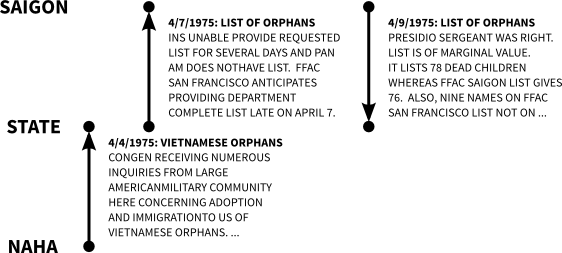
\includegraphics[width=\textwidth]{../fig/cables_orphan_example.png}
% \caption{Example excerpts of cables sent in April 1975 concerning orphans from the Vietnam War.}
% \label{fig:cables_example}
% \end{figure}

\parhead{arXiv}

\parhead{Enron}


\PP insert table and refetence for both (number of days, entities, total messages, or something); maybe a plot showing attributes of the data...somehow inform them that the state department is a bias for the cables data

\PP footnote on handling multiple recipients of message...

\subsection{Metrics and competing methods}

\PP how we evaluate based on real events

\PP how we evaluate based on perplexity (prediction of words)

\PP competing methods for perplexity: LDA, average user words?, dynamic topic model, network topic models

\subsection{Performance and exploration}

\PP sumry of comparison to gold-standard events for cables

\PP table of predictive likelihood results and summary pgh; and/or cite tea leaves paper

\parhead{Exploration}

\PP charachetrize events manually (based on cables) vs event detection characterization

\PP show descriptions for cables entities and select events; same for arxiv/enron

\PP any other exploration you can think of!


Results: ROC curve (x=false postive rate, y=true postive rate)